\subsection{代数式}\label{subsec:2-1}

\begin{enhancedline}
在小学里我们已经知道,可以用字母表示数。
例如,长方形的面积可以写成:
$$ S = ab \,\douhao $$
这里字母 $S$ 表示长方形的面积,字母$a$,$b$ 分别表示长方形的长和宽。

我们知道,数的运算律可以用字母简明地写成:\\
\hspace*{4em}\begin{tblr}{colspec={Q[l,7em] Q[l,$]}, colsep=0pt, rowsep=0pt}
    加法交换律 &  a + b = b + a; \\
    加法结合律 & (a + b) + c = a + (b + c); \\
    乘法交换律 & ab = ba; \\
    乘法结合律 & (ab)c = a(bc); \\
    分配律    & a(b + c) = ab + ac \,\juhao
\end{tblr}\\
这里字母 $a$,$b$,$c$ 表示任意的有理数。

在代数里,我们常常用字母表示数。

例如,汽车每小时走 40 千米,那么 2 小时, 2.5 小时,
$1\dfrac{3}{4}$ 小时所走的千米数就分别是:
$$ 40 \times 2,\quad 40 \times 2.5,\quad 40 \times 1\dfrac{3}{4} \juhao $$

如果用字母 $t$ 表示汽车行驶的小时数,那么汽车所走的千米数就是
$$ 40t \,\juhao $$

如果用字母 $v$ 表示汽车每小时所走的千米数,$t$ 表示汽车行驶的小时数,
那么汽车所走的千米数就是
$$ vt \,\juhao $$

从上面的例子可以看出,用字母表示数,能够把数量或数量关系一般地而又简明地表达出来。

在上面的一些例子里,我们得到许多含有字母的式子 如 $ab$,\, $a + b$,\, $40t$,\, $vt$,等等。
象这样用运算符号\footnote{这里的运算是指加、减、乘、除、乘方、开方。开方运算以后讲。}
把数或表示数的字母连结而成的式子,叫做\zhongdian{代数式}。

单独的一个数或者一个字母,象 $-31$,\, $0$,\, $x$,也是代数式。

代数式里的每个字母都表示数,因此,数的一些运算规律也适用于代数式。

用代数式表示一些数量或数量关系,对以后的学习非常重要。


\liti 用代数式表示:

\begin{xiaoxiaotis}
    \begin{tblr}{columns={18em, colsep=0pt}, stretch=1.2}
        \xxt{$x$ 与 5 的差;}         & \xxt{$b$ 除以 8 的商;} \\
        \xxt{$x$ 的 $\dfrac{1}{3}$;} & \xxt{$y$ 的 $50\%$。} \\
    \end{tblr}
\end{xiaoxiaotis}

\begin{xiaoxiaotis}
    \resetxxt
    \jie \begin{tblr}[t]{columns={10em, l, colsep=0pt}, stretch=1.5}
        \xxt{$x - 5$;}         & \xxt{$\dfrac{b}{8}$;} \\
        \xxt{$\dfrac{1}{3}x$;} & \xxt{$\dfrac{50}{100}y$。} \\
    \end{tblr}\jiange
\end{xiaoxiaotis}

\begin{wrapfigure}[3]{r}{6cm}
    \centering
    \begin{tikzpicture}
        \draw (0, 0) rectangle (4, 2);
        \node at (2, -0.3) {$a$};
        \node at (4.2, 1) {$b$};
    \end{tikzpicture}
    \caption{}\label{fig:2-1}
\end{wrapfigure}

\liti 根据图 \ref{fig:2-1},求长方形的周长 $l$。

\jie $\begin{aligned}[t]
    l &= a \times 2 + b \times 2 \\
        &= 2a + 2b \juhao
\end{aligned}$

\zhuyi 数和表示数的字母相乘时,如果省略乘号,应当把数写在字母的前面,如 $a \times 2$ 应写成 $2a$, 不写成 $a2$ 。

\lianxi
\begin{xiaotis}

\xiaoti{用代数式表示:}
\begin{xiaoxiaotis}

    \begin{tblr}{columns={18em, colsep=0pt}}
        \xxt{$15$ 与 $S$ 的和;}    & \xxt{$x$ 与 $3$ 的差;} \\
        \xxt{$a$ 乘以 $15$ 的积;}  & \xxt{$a$ 除以 $15$ 的商;} \\
        \xxt{$y$ 的 $70\%$;}       & \xxt{$d$ 的 $a$ 倍的 $\dfrac{2}{3}$。} \\
    \end{tblr}

\end{xiaoxiaotis}

\xiaoti{填写下表:\jiange}

% 下表中,使用 minipage 是为了让元素能够(竖直)居中显示。
\def\lena{5em}
\def\lenb{2.5cm}
\def\lend{6em}
\begin{longtblr}[theme=nocaption]{
    hlines, vlines,
    colspec={cclcc},
    cells={valign=m},
    row{2, 9}={ht=3em},
    rowhead = 1,
}
    名称 & 图形 &  文字表示的公式 & 字母的意义 & {字母表示\\的公式} \\
    \SetCell[r=2]{m, \lena}长方形
         & \SetCell[r=2]{m, \lenb}{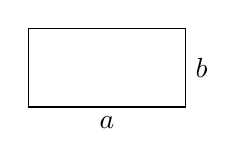
\begin{tikzpicture}
            \draw (0, 0) rectangle (2, 1);
            \node at (1, -0.2) {$a$};
            \node at (2.2, 0.5) {$b$};
          \end{tikzpicture}}
        & $\text{周长} = \text{长} \times 2 + \text{宽} \times 2$
        & \SetCell[r=2]{l, \lend}{
            $l$ —— 周长 \\
            $S$ —— 面积 \\
            $a$ —— 长 \\
            $b$ —— 宽}
        & $l = 2a + 2b$ \\
    & & $\text{面积} = \text{长} \times \text{宽}$ & & $S = ab$ \\
    \SetCell[r=2]{m, \lena}正方形
         & \SetCell[r=2]{m, \lenb}{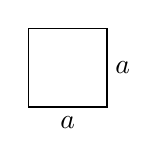
\begin{tikzpicture}
            \draw (0, 0) rectangle (1, 1);
            \node at (0.5, -0.2) {$a$};
            \node at (1.2, 0.5) {$a$};
          \end{tikzpicture}}
        & $\text{周长} = \text{边长} \times 4$
        & \SetCell[r=2]{l, \lend}{
            $l$ —— 周长 \\
            $S$ —— 面积 \\
            $a$ —— 边长}
        & \vspace*{0.5em}  \\
    & & $\text{面积} = \text{边长}^2$ & \\
    三角形
        & \begin{minipage}[c]{\lenb}\begin{tikzpicture}
            \draw (0, 0) -- (2, 0) -- (1.3, 1) -- cycle;
            \draw (1.3, 1) to[chuizu] node[pos=0.5, left, inner sep=0.1em] {$h$} (1.3, 0);
            \node at (1, -0.2) {$a$};
          \end{tikzpicture} \end{minipage}
        & $\text{面积} = \dfrac{1}{2} \times \text{底} \times \text{高}$
        & \begin{minipage}[c][5em]{\lend}
            $S$ —— 面积 \\
            $a$ —— 底 \\
            $h$ —— 高
          \end{minipage}
        & \\
    {平行\\四边行}
        & \begin{minipage}[c]{\lenb}\begin{tikzpicture}
            \draw (0, 0) -- (2, 0) -- (2.4, 1) -- (0.4, 1) -- cycle;
            \draw (0.4, 1) to[chuizu] node[pos=0.5, right, inner sep=0.1em] {$h$} (0.4, 0);
            \node at (1, -0.2) {$a$};
          \end{tikzpicture} \end{minipage}
        & $\text{面积} = \text{底} \times \text{高}$
        & \begin{minipage}[c][5em]{\lend}
            $S$ —— 面积 \\
            $a$ —— 底 \\
            $h$ —— 高
          \end{minipage}
        & \\
    梯形
        & \begin{minipage}[c]{\lenb}\begin{tikzpicture}
            \draw (0, 0) -- (2, 0) -- (1.2, 1) -- (0.4, 1) -- cycle;
            \draw (0.4, 1) to[chuizu] node[pos=0.5, right, inner sep=0.1em] {$h$} (0.4, 0);
            \node at (0.8, 1.2) {$a$};
            \node at (1, -0.2) {$b$};
          \end{tikzpicture} \end{minipage}
        & $\text{面积} = \dfrac{1}{2} \times (\text{上底} + \text{下底}) \times \text{高}$
        & \begin{minipage}[c][7em]{\lend}
            $S$ —— 面积 \\
            $a$ —— 上底 \\
            $b$ —— 下底 \\
            $h$ —— 高
          \end{minipage}
        & \\
    \SetCell[r=2]{m, \lena}{圆}
        & \SetCell[r=2]{m, \lenb}{\begin{tikzpicture}[>=Stealth]
            \pgfmathsetmacro{\r}{1}
            \draw (0, 0) circle (\r);
            \draw (-1.2*\r, 0) -- (-\r, 0)
                 (\r, 0) -- (1.2*\r, 0);
            \draw [dashed] (-\r, 0) -- (\r, 0);
            \draw (0, -1.2*\r) -- (0, -\r)
                (0, \r) -- (0, 1.2*\r);
            \draw [dashed] (0, -\r) -- (0, \r);
            \draw [->] (0, 0) -- (30:1) node [pos=0.5, above left, inner sep=0.1em] {$r$};
         \end{tikzpicture}}
       & $\text{周长} = 2 \times \text{圆周率} \times \text{半径}$
       & \SetCell[r=2]{l, \lend}{
           $C$ —— 周长 \\
           $S$ —— 面积 \\
           $\pi$ —— 圆周率 \\
           $r$ —— 半径}
       & \\*
   & & $\text{面积} = \text{圆周率} \times \text{边长}^2$ & \\
\end{longtblr}

\end{xiaotis}

\lianxijiange

\liti 用代数式表示:
\begin{xiaoxiaotis}

    \xxt{$x$ 与 $-1$ 的和的 $\dfrac{2}{5}$;}

    \xxt{比 $a$ 的 $\dfrac{5}{9}$ 大 $4$ 的数;}

    \xxt{比 $m$ 的相反数少 $5$ 的数;}

    \xxt{比 $n$ 的倒数大 $2$ 的数。}

\end{xiaoxiaotis}

\begin{xiaoxiaotis}
    \resetxxt
    \jie  \begin{tblr}[t]{columns={18em, l, colsep=0pt}, stretch=1.5}
        \xxt{$\dfrac{2}{5} (x - 1)$;}    & \xxt{$\dfrac{5}{9}a + 4$;} \\
        \xxt{$-m - 5$;} & \xxt{$\dfrac{1}{n} + 2$。} \\
    \end{tblr}
\end{xiaoxiaotis}


\liti 设某数为 $x$,用代数式表示:
\begin{xiaoxiaotis}

    \xxt{某数与 $3$ 的和的 $3$ 倍;}

    \xxt{$4$ 除以某数平方的商减 $-5$ 的差。}

    \resetxxt
    \jie \twoInLineXxt{$3 (x + 3)$;}{$\dfrac{4}{x^2} + 5$。}

\end{xiaoxiaotis}


\liti 设甲数为 $x$,乙数为 $y$,用代数式表示:
\begin{xiaoxiaotis}

    \xxt{甲乙两数的平方和;}

    \xxt{甲乙两数的和与甲乙两数的差的积。}

    \resetxxt
    \jie  \twoInLineXxt{$x^2 + y^2$;}{$(x + y) (x - y)$。}
\end{xiaoxiaotis}


\liti 设甲数为 $x$,用代数式表示乙数;
\begin{xiaoxiaotis}

    \xxt{乙数比甲数多 $5$;}

    \xxt{甲乙两数的和为 $16$。}

    \resetxxt
    \jie  \twoInLineXxt{$x + 5$;}{$16 - x$。}
\end{xiaoxiaotis}


\lianxi
\begin{xiaotis}

\xiaoti{用代数式表示:}
\begin{xiaoxiaotis}

    \xxt{$a$ 与 $-8$ 的差的 $2$ 倍 ;}

    \xxt{$x$ 的 $5\%$ 与 $y$ 的 $6\%$ 的和;}

    \xxt{比 $x$ 的倒数小 $8$ 的数;}

    \xxt{比 $a$ 的 $\dfrac{3}{4}$ 多 $b$ 的数。}

\end{xiaoxiaotis}


\xiaoti{设某数为 $x$,用代数式表示:}
\begin{xiaoxiaotis}

    \xxt{某数的 $8$ 倍与 $7$ 的和;}

    \xxt{某数的立方的 $3$ 倍与 $-3$ 的差;}

    \xxt{$5$ 与某数的差的 $2$ 倍;}

    \xxt{某数除以 $2$ 的商与 $7$ 的差。}

\end{xiaoxiaotis}


\xiaoti{用代数式表示:}
\begin{xiaoxiaotis}

    \xxt{$a$ 与 $b$ 的和乘以 $c$;}

    \xxt{$a$ 与 $b$ 的差的平方;}

    \xxt{$a$,$b$ 两数的平方差;}

    \xxt{$a$,$b$ 的积除以 $a$,$b$ 的差。}

\end{xiaoxiaotis}


\xiaoti{设甲数为 $x$,乙数为 $y$,用代数式表示:}
\begin{xiaoxiaotis}

    \xxt{甲数与乙数的和的绝对值;}

    \xxt{甲数的 $2$ 倍与乙数的和乘以甲数的 $2$ 倍与乙数的差。}

\end{xiaoxiaotis}


\xiaoti{设甲数为 $x$,用代数式表示乙数:}
\begin{xiaoxiaotis}

    \xxt{乙数比甲数的 $2$ 倍少 $6$;}

    \xxt{甲乙两数的差为 $15$。}

\end{xiaoxiaotis}

\end{xiaotis}
\lianxijiange

\begin{wrapfigure}[6]{r}{6cm}
    \centering
    \begin{tikzpicture}[>=Stealth]
        \filldraw [fill=gray!50]  (0, 0) rectangle (3, 3);
        \filldraw [fill=white] (1, 1) rectangle (2, 2);
        \draw [<->] (1, 1.2) -- (2, 1.2) node [midway, inner sep=1pt, fill=white] {$b$};
        \draw [<->] (0, -0.2) to[xianduan] node [midway, inner sep=1pt, fill=white] {$a$} (3, -0.2);
    \end{tikzpicture}
    \caption{}\label{fig:2-2}
\end{wrapfigure}


\liti 如图 \ref{fig:2-2} , 垫铁的外正方形的边长是 $a$ 毫米,
内正方形的边长是 $b$ 毫米,用代数式表示阴影部分的面积。

\jie 边长是 $a$ 毫米的正方形的面积是 $a^2$ 平方毫米;
     边长是 $b$ 毫米的正方形的面积是 $b^2$ 平方毫米。

所以,阴影部分的面积是 $(a^2 - b^2)$ 平方亳米。

\liti 甲乙两地之间公路全长 245 千米,从甲地乘汽车到乙地,每小时走 $v$ 千米,用代数式表示:
\begin{xiaoxiaotis}

    \xxt{汽车从甲地到乙地需要走多少小时;}

    \xxt{如果每小时加快 3 千米, 需要走多少小时;}

    \xxt{加快速度后可以早到多少小时,}

    \resetxxt
    \jie \xxt{汽车从甲地到乙地需要走 $\dfrac{245}{v}$ 小时;}

    \xxt{如果每小时加快 3 千米, 需要走 $\dfrac{245}{v + 3} $小时;}

    \xxt{加快速度后可以早到 $\left(\dfrac{245}{v} - \dfrac{245}{v+3}\right)$ 小时。}

\end{xiaoxiaotis}


\lianxi
\begin{xiaotis}

\xiaoti{写出示下列各种零件断面(阴影部分)面积的代数式:}

\begin{figure}[htbp]
    \centering
    \begin{tikzpicture}[>=Stealth, scale=0.9]
    \begin{scope}
        \draw [pattern={mylines[angle=45, distance={5pt}]}] (0, 0) circle (2);
        \draw [fill=white] (0, 0) circle (1);
        \draw [loosely dash dot] (2.5, 0) -- (-2.5, 0) (0, -2.5) -- (0, 2.5);
        \draw [->] (0, 0) -- (120:2) node [pos=0.3, left] {$R$};
        \draw [->] (0, 0) -- (320:1) node [pos=0.3, right] {$r$};
        \node at (0, -3) {(1)};
    \end{scope}

    \begin{scope}[xshift=4cm, every node/.style={fill=white}]
        \draw [pattern={mylines[angle=135, distance={5pt}]}] (0, -2) rectangle (6, 2);
        \draw [fill=white] (1, -1) rectangle (5, 1);
        \draw [<->] (0, 0) -- (1, 0) node [midway, above] {$x$};
        \draw [<->] (5, 0) -- (6, 0) node [midway, above] {$x$};
        \draw [<->] (3, -2) -- (3, -1) node [midway, right] {$x$};
        \draw [<->] (3,  2) -- (3,  1) node [midway, right] {$x$};
        \draw [<->] (0, -2.4) to [xianduan={above=1em}] node [midway] {30} (6, -2.4);
        \draw [<->] (6.4, -2) to [xianduan={above=1em}] node [midway] {20} (6.4, 2);
        \node at (3, -3) {(2)};
    \end{scope}
\end{tikzpicture}

    \caption*{(第 1 题)}
\end{figure}

\xiaoti{有 $m$ 公顷水稻要收割,原计划每天收割 $S$ 公顷,解放军来支援,
    每天多收割 5 公顷。用代数式表示:
}
\begin{xiaoxiaotis}

    \xxt{按原计划多少天割完;}

    \xxt{解放军支援后,多少天割完;}

    \xxt{解放军支援后,提前几天割完。}
\end{xiaoxiaotis}

\xiaoti{某班同学共 50 人,在“学雷铎” 活动中,有五分之四的同学每人做好事 $a$ 件,
    其余同学每人做好事比 $a$ 件多 1 件,用代数式表示全班同学共做好事多少件。
}

\end{xiaotis}
\lianxijiange


\liti 用代数式表示:

(1) 含盐 18 的盐水 $a$ 千克,其中含纯盐多少千克;

(2) 浓度为 $75\%$ 的酒精溶液 $x$ 克,其中含纯酒精多少克,含水多少克。

说明: “含盐 $18\%$ 的盐水”,就是指 1 千克这样的盐水中,含纯盐 $\dfrac{18}{100}$ 千克;

“浓度为 $75\%$ 的酒精溶液”,就是指 1 克这样的酒精溶液中,含纯酒精 $\dfrac{75}{100}$ 克。

\jie (1)$a$ 千克这样的盐水中,含纯盐 $\dfrac{18}{100}a$ 千克;

(2) $x$ 克这样的酒精溶液中,含纯酒精 $\dfrac{75}{100}x$克,含水 $\left(x - \dfrac{75}{100}x\right)$ 克。


\lianxi
\begin{xiaotis}

\xiaoti{用代数式表示:}
\begin{xiaoxiaotis}

    \xxt{含盐 $25\%$ 的盐水 $m$ 千克,含纯盐多少千克,含水多少千克;}

    \xxt{浓度为 $72\%$ 的硫酸溶液 $y$ 千克,含纯硫酸多少千克,含水多少千克。}

\end{xiaoxiaotis}

\xiaoti{原有水田 26 公顷,现在比原来增加 $75\%$,现有水田多少公顷?}

\xiaoti{稻谷的出米率一般是 $72\%$, 现有稻谷 $(G + 10)$ 千克,能加工出大米多少千克?}

\end{xiaotis}
\end{enhancedline}
